\documentclass{article}
\usepackage[paperwidth=841mm, paperheight=1189mm, margin=20mm]{geometry}
\usepackage{lmodern}
\usepackage[sfdefault, lining]{FiraSans}
\usepackage[table]{xcolor}
\usepackage{graphicx}
\usepackage{booktabs}
\usepackage{adjustbox}
\usepackage{amsmath}
\usepackage{amssymb}
\usepackage[hidelinks]{hyperref}
\usepackage{qrcode}
\usepackage{enumitem}
\usepackage{ragged2e}
\usepackage[most]{tcolorbox}
\usepackage{tikz}
\usetikzlibrary{svg.path}

\definecolor{navy}{RGB}{12,45,87}
\definecolor{accent}{RGB}{26,99,176}
\definecolor{numeral}{RGB}{150,184,224}
\definecolor{leaf}{RGB}{0,160,64}
\definecolor{pagebg}{RGB}{241,245,249}
\definecolor{rowtint}{RGB}{236,242,249}
\definecolor{rule}{RGB}{206,216,228}
\definecolor{ink}{RGB}{28,36,46}
\definecolor{muted}{RGB}{88,100,116}

\pagestyle{empty}
\setlength{\parindent}{0pt}
\setlength{\parskip}{0pt}
\hyphenpenalty=10000
\exhyphenpenalty=10000

\newcommand{\bodysize}{\fontsize{26}{34}\selectfont}
\newcommand{\tablesize}{\fontsize{23}{30}\selectfont}
\newcommand{\notesize}{\fontsize{20}{26}\selectfont}
\newcommand{\hl}[1]{\textbf{\textcolor{accent}{#1}}}
\newcommand{\fittable}[1]{{\tablesize\rowcolors{2}{rowtint}{white}\adjustbox{max width=\linewidth}{\input{#1}}}}
\newcommand{\srcnote}[1]{\par\vspace{4mm}{\centering\notesize\textcolor{muted}{#1}\par}}
\newcommand{\sub}[1]{\par\vspace{3mm}{\bfseries\textcolor{navy}{#1}}\par\vspace{1mm}}

\setlist[itemize]{leftmargin=1.1em, itemsep=2.5mm, topsep=2mm, parsep=0pt,
  label={\textcolor{navy}{\textbullet}}}
\setlist[itemize,2]{leftmargin=1.1em, itemsep=1mm, topsep=1mm,
  label={\textcolor{muted}{--}}}

\newtcolorbox{block}[2][]{enhanced, arc=4mm,
  colback=white, colframe=white, boxrule=0pt,
  colbacktitle=navy, coltitle=white,
  fonttitle=\bfseries\fontsize{38}{46}\selectfont,
  toptitle=2mm, bottomtitle=2mm, left=9mm, right=9mm, top=6mm, bottom=6mm,
  title={#2}, fontupper=\bodysize\color{ink}\RaggedRight, #1}

\newcommand{\closing}[2]{\par\vspace{8mm}{\color{leaf}\rule{28mm}{1.4mm}}\par
  \vspace{4mm}{\bfseries\textcolor{navy}{#1}}\hspace{0.4em}#2\par}

\newcommand{\sectitle}[2]{\tikz[baseline=(n.base)]\node[circle, fill=leaf,
  text=white, inner sep=0pt, minimum size=1.08em, font=\bfseries\fontsize{32}{32}\selectfont](n){#1};\hspace{0.5em}#2}

\begin{document}
\pagecolor{pagebg}
\bodysize\color{ink}

\begin{tcolorbox}[enhanced, colback=navy, colframe=navy, arc=4mm, boxrule=0pt,
  left=12mm, right=12mm, top=8mm, bottom=8mm]
  \begin{minipage}[c]{0.13\linewidth}\centering
    
\includegraphics[width=0.92\linewidth]{assets/ncu-logo.png}
  \end{minipage}\hfill
  \begin{minipage}[c]{0.70\linewidth}\centering\color{white}
    {\bfseries\fontsize{76}{90}\selectfont Hierarchical Projection as a Validity Layer\\
      for Multilingual ESG Promise Verification\par}
    \vspace{5mm}{\color{leaf}\rule{40mm}{1.6mm}}\par\vspace{5mm}
    {\fontsize{40}{50}\selectfont Sheng-Xun Chen, Chun-Wei Chen, Hsin-Chen Han,
      Shi-Yu Huang\par}
    \vspace{4mm}
    {\fontsize{31}{40}\selectfont National Central University, Taiwan
      \quad\textcolor{leaf}{$\bullet$}\quad Team\_10537\par
      NTCIR-19 AI CUP Special Session
      \quad\textcolor{leaf}{$\bullet$}\quad VeriPromiseESG Task\par}
  \end{minipage}\hfill
  \begin{minipage}[c]{0.13\linewidth}\centering
    \definecolor{ntcirletter}{RGB}{255,255,255}
    \definecolor{ntcirleaf}{RGB}{0,160,64}
    \resizebox{0.96\linewidth}{!}{% NTCIR logo, path data copied from the SVG in the header of
% https://research.nii.ac.jp/ntcir/ntcir-19/index.html (viewBox 0 0 437 176).
\providecolor{ntcirletter}{RGB}{0,56,141}
\providecolor{ntcirleaf}{RGB}{0,160,64}
\begin{tikzpicture}[yscale=-1, line width=0pt]
  \fill[fill=ntcirletter] svg {M0.792847 175.511H11.4833V61.9579C11.4833 61.9579 55.6414 144.046 67.2456 165.38C68.9632 168.538 71.4167 171.711 71.4267 171.72C71.5039 171.787 73.4284 174.66 80.7869 175.263C88.1455 175.866 90.0252 169.17 90.1728 168.559C90.3204 167.948 90.4051 167.398 90.4051 167.398L90.4847 52.3207L80.8819 52.1879L79.4064 163.762C79.4064 163.762 20.9633 55.8619 20.7084 55.505C20.4534 55.1478 17.6813 50.7837 9.4777 51.2682C1.27409 51.7527 0.792847 58.5481 0.792847 58.5481V175.511Z};
  \fill[fill=ntcirletter] svg {M106.793 53.6951L106.803 63.1847L144.883 63.2029L144.725 175.599H155.796L156.136 62.9939L193.393 62.8306V53.6951H106.793Z};
  \fill[fill=ntcirletter] svg {M278.711 54.5437L278.476 63.7278C278.298 63.7616 268.178 62.5657 254.301 64.2428C243.701 65.5238 231.028 68.8232 222.281 76.5246C212.145 85.4489 205.121 95.148 205.468 112.998C206.594 171.051 263.392 165.909 279.064 165.448L279.221 174.363C279.221 174.363 276.957 175.072 270.738 175.17C269.732 175.185 267.331 175.138 266.188 175.17C253.857 175.509 235.302 173.023 220.021 163.575C205.568 154.641 192.8 139.876 193.414 112.675C193.888 91.6845 202.3 79.2867 212.581 70.4597C222.019 62.3572 232.954 57.4703 243.684 55.599C263.091 52.2146 278.598 54.5437 278.711 54.5437Z};
  \fill[fill=ntcirletter] svg {M352.896 175.599H363.92L363.777 82.1216C363.777 82.1216 365.425 61.842 391.083 61.6434C416.742 61.4451 423.953 77.0315 423.748 84.1793C423.543 91.3274 419.523 108.899 400.564 108.899C381.603 108.899 367.999 108.898 367.999 108.898L367.797 117.735L406.025 118.43C406.025 118.43 424.574 118.628 426.117 136.796L426.465 175.599H436.731L436.318 134.116C436.318 134.116 434.775 114.856 419.11 112.374C419.11 112.374 426.4 109.249 430.944 100.786C433.164 96.6501 434.635 90.9588 434.465 84.2786C434.335 79.1219 433.083 75.0591 431.095 70.9375C425.238 58.7929 411.998 50.87 394.38 50.4252C370.784 49.8294 353.835 65.08 352.907 82.9501C351.978 100.82 352.896 175.599 352.896 175.599Z};
  \fill[fill=ntcirletter] svg {M304.145 53.6951H314.338L313.78 175.599H303.414L304.145 53.6951Z};
  \fill[fill=ntcirleaf] svg {M288.979 50.8094C288.979 50.8094 290.231 52.0714 291.934 50.4081C294.365 48.0369 298.466 42.5795 305.097 39.8702C313.235 36.5463 323.956 38.931 332.444 33.1341C341.156 27.1838 347.537 12.9373 348.155 0.528564C348.155 0.528564 340.417 5.40502 332.315 5.83457C316.251 6.68607 294.861 14.1303 296.01 39.5491C296.01 39.5491 291.856 42.5743 289.193 49.799C288.847 50.7351 288.971 50.8502 288.979 50.8094Z};
\end{tikzpicture}
}
  \end{minipage}
\end{tcolorbox}

\vspace{9mm}

\begin{tcbraster}[raster columns=2, raster equal height=rows,
  raster column skip=10mm, raster row skip=9mm]
\begin{block}{\sectitle{1}{Introduction}}
  \begin{itemize}
    \item ESG promise verification labels each paragraph with \textbf{four linked
      fields}, and the output is meant for audit-oriented use.
    \item A record is only usable if its fields agree, yet independent
      classifiers can combine plausible labels into an impossible tuple.
    \item The official metric scores each field on its own, so an invalid
      tuple still earns \textbf{44.3\%} of the weighted field credit.
  \end{itemize}
  \closing{Research question.}{\itshape Can a retraining-free decision rule
    guarantee legal outputs, and how does it change field-wise versus
    whole-tuple scores?}
\end{block}
\begin{block}{\sectitle{2}{Task \& Data}}
  \begin{itemize}
    \item Fields: promise status (PS), verification timeline (VT), evidence
      status (ES), evidence quality (EQ).
    \item Hard rules: PS\,=\,No $\Rightarrow$ VT\,=\,ES\,=\,EQ\,=\,N/A;\\
      ES\,=\,No $\Rightarrow$ EQ\,=\,N/A.
    \item Only \textbf{17 of 120} label combinations are legal.
    \item \textbf{AI CUP 2026}: 2,000 Chinese paragraphs from 49 reports, all
      legal (15 of 17 states observed).
    \item \textbf{ML-Promise}: English, French, Japanese (400 paragraphs each),
      Korean (500 PDF pages).
  \end{itemize}
\end{block}
\end{tcbraster}

\vspace{9mm}

\begin{block}{\sectitle{3}{Methodology}}
  \begin{minipage}[t]{0.50\linewidth}\vspace{0pt}
    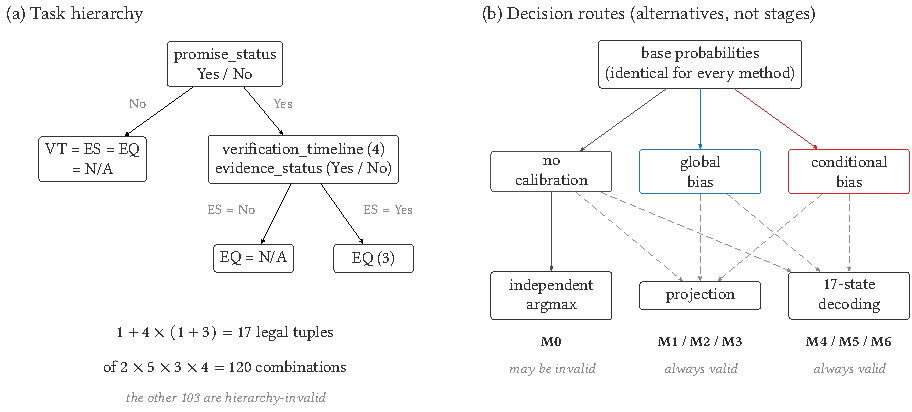
\includegraphics[width=\linewidth]{../figures/figure1_hierarchy.pdf}
    \srcnote{Figure 1: the label hierarchy and the seven alternative decision
      rules, all reading the same base probabilities}
  \end{minipage}\hfill
  \begin{minipage}[t]{0.465\linewidth}\vspace{0pt}
    \sub{Validity-preserving output rules}
    \begin{itemize}
      \item \textbf{\textcolor{navy}{Projection}}: greedy and top-down. Pick PS; under PS\,=\,Yes take
        the best substantive VT and ES; under ES\,=\,Yes the best substantive
        EQ. Always legal, no retraining.
      \item \textbf{\textcolor{navy}{17-state decoding}}: return the legal state with the highest
        summed log-score.
      \item Calibration: none, global, or conditional class biases.
    \end{itemize}
    \sub{Evaluation}
    \begin{itemize}
      \item \texttt{\fontsize{24}{30}\selectfont hfl/chinese-roberta-wwm-ext-large},
        four independent heads.
      \item Five-way cross-fitting, three seeds, document-disjoint split.
      \item Paired report-cluster bootstrap, Holm-adjusted.
      \item External: 4 backbones $\times$ $\lambda\in\{0,0.3\}$ in each of 4
        languages = \textbf{32 arms}.
    \end{itemize}
  \end{minipage}
\end{block}

\vspace{9mm}

\begin{block}{\sectitle{4}{Results: Chinese Anchor}}
  \begin{minipage}[t]{0.575\linewidth}\vspace{0pt}
    \centering\fittable{../tables/table2_main.tex}
    \srcnote{Table 2: three-seed means $\pm$ s.d., document-disjoint}
  \end{minipage}\hfill
  \begin{minipage}[t]{0.395\linewidth}\vspace{0pt}
    \centering\fittable{../tables/table4_contrasts.tex}
    \srcnote{Table 4: pre-specified paired contrasts, 95\% intervals}
  \end{minipage}
  \par\vspace{6mm}
  \begin{itemize}
    \item Projection removes every invalid tuple (\hl{12.55\% $\to$ 0}) and
      raises tuple accuracy by \hl{+0.035} ($p_{\mathrm{Holm}}=.001$), while
      official wF1 does not move ($\Delta=-0.001$, $p_{\mathrm{Holm}}=1.000$).
    \item Searching all 17 states is not better: joint decoding loses
      \hl{$-$0.006} tuple accuracy to projection ($p_{\mathrm{Holm}}=.028$).
  \end{itemize}
\end{block}

\vspace{9mm}

\begin{tcbraster}[raster columns=2, raster equal height=rows,
  raster column skip=10mm, raster row skip=9mm]
\begin{block}{\sectitle{5}{Multilingual Replication}}
  {\centering\fittable{../tables/table7_multilingual_mechanism.tex}\par}
  \srcnote{Table 7: projection (M1) vs.\ argmax (M0), one preselected arm per
    corpus}
  \begin{itemize}
    \item Tuple accuracy rises in \hl{32/32} external arms; wF1 in only
      \hl{14/32} (EN 7/8, FR 5/8, JA 0/8, KO 2/8).
    \item These are within-arm directions, not a ranking of languages.
  \end{itemize}
\end{block}
\begin{block}{\sectitle{6}{Why the Metrics Disagree}}
  \begin{itemize}
    \item A wrong parent makes projection overwrite a correct child with N/A;
      a right parent lets it repair an unsupported child.
    \item N/A credit goes up and substantive credit goes down in all five
      corpora, yet whole tuples improve in every one.
    \item Joint decoding revises PS on \textbf{339 of 12,000} rows: 225 become
      correct and 114 wrong, but whole-row correctness on them falls
      \textbf{114 $\to$ 47}.
    \item Fixing a parent rarely saves a row whose children stay wrong;
      breaking a correct parent always loses it.
  \end{itemize}
\end{block}
\begin{block}{\sectitle{7}{Implications for Audit Use}}
  \begin{itemize}
    \item Validity is a \textbf{precondition} for a usable record, not proof that
      the record is right.
    \item A repair can hide an inconsistency, so a deployed validity layer
      should \textbf{log the rows it repaired}.
    \item Pick the metric by how outputs are used:
      \begin{itemize}
        \item records: tuple accuracy among valid outputs
        \item single-field actions: that field's F1, or rare-class recall
        \item portfolio statistics: class-level scores, keeping validity
        \item leaderboards: official wF1, but not for gaps under 0.008
      \end{itemize}
  \end{itemize}
\end{block}
\begin{block}{\sectitle{8}{Conclusion}}
  \begin{itemize}
    \item Hierarchical projection is a \textbf{retraining-free validity layer}: it
      eliminates invalid tuples by construction.
    \item It improves whole-tuple accuracy on the Chinese anchor and in all 32
      external arms.
    \item Its field-score effect varies across models and corpora; its logical
      guarantee does not.
  \end{itemize}
  \closing{Takeaway.}{For audit use, make validity a precondition, and pick
    the metric that matches the unit at which errors have consequences.}
\end{block}
\end{tcbraster}

\vfill

\begin{tcolorbox}[enhanced, colback=navy, colframe=navy, arc=4mm, boxrule=0pt,
  left=12mm, right=12mm, top=7mm, bottom=7mm]
  \begin{minipage}[c]{0.66\linewidth}\notesize\color{white}\RaggedRight
    {\bfseries References}\par\vspace{2mm}
    \begin{enumerate}[label={\textcolor{numeral}{[\arabic*]}}, leftmargin=2.2em,
      itemsep=0.6mm, topsep=0pt, parsep=0pt]
      \item AI CUP 2026 Organizers. ESG Sustainability Commitment Verification
        Competition 2026 (VeriPromiseESG4K). 2026.
      \item M.-Y. Day et al. VeriPromiseESG4K: A Traditional Chinese ESG Promise
        Verification Dataset for AI CUP 2026. IEEE IRI, 2026.
      \item C.-C. Chen et al. SemEval-2025 Task 6: Multinational, Multilingual,
        Multi-Industry Promise Verification. SemEval, 2025.
      \item Y. Seki et al. ML-Promise: A Multilingual Dataset for Corporate
        Promise Verification. EMNLP, 2025.
    \end{enumerate}
  \end{minipage}\hfill
  \begin{minipage}[c]{0.20\linewidth}\RaggedLeft\color{white}
    {\bfseries\fontsize{26}{32}\selectfont Code \& reproduction\par}
    \vspace{4mm}
    {\fontsize{19}{24}\selectfont\href{https://github.com/tom1030507/ntcir19-esg-validity-layer}{github.com/tom1030507/\\ntcir19-esg-validity-layer}\par}
  \end{minipage}\hspace{8mm}
  \begin{minipage}[c]{0.11\linewidth}\centering
    \href{https://github.com/tom1030507/ntcir19-esg-validity-layer}{\XeTeXLinkBox{\colorbox{white}{\qrcode[height=4.6cm, nolink]{https://github.com/tom1030507/ntcir19-esg-validity-layer}}}}
  \end{minipage}
\end{tcolorbox}

\end{document}
